
\begin{minipage}[t]{\textwidth}
\Aufgabe{Struktogramme und Klassendiagramme}

\textbf{Setze folgende Diagramme in BlueJ-Blockly um und notiere den Programmcode auf der nächsten Seite}

\vspace{0.5cm}

\doppelseite{0.45}{0.5}{t}{%
\textbf{Klassendiagramm:}

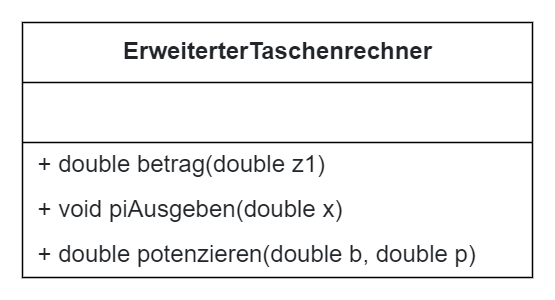
\includegraphics[width=\linewidth]{_Aufgaben/BlocksAndJava/img/klasse.png} 
}{%

\textbf{Struktogramm für piAusgeben(double x):}

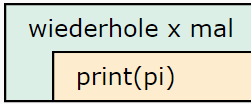
\includegraphics[width=0.6\linewidth]{_Aufgaben/BlocksAndJava/img/strukt_10pi.png}
}

\vspace{1cm}

\textbf{Zeichne hier die Struktogramme für die restlichen Methoden:}

\LoesungKaro{\\
\Large
+ double betrag(double z1) \\
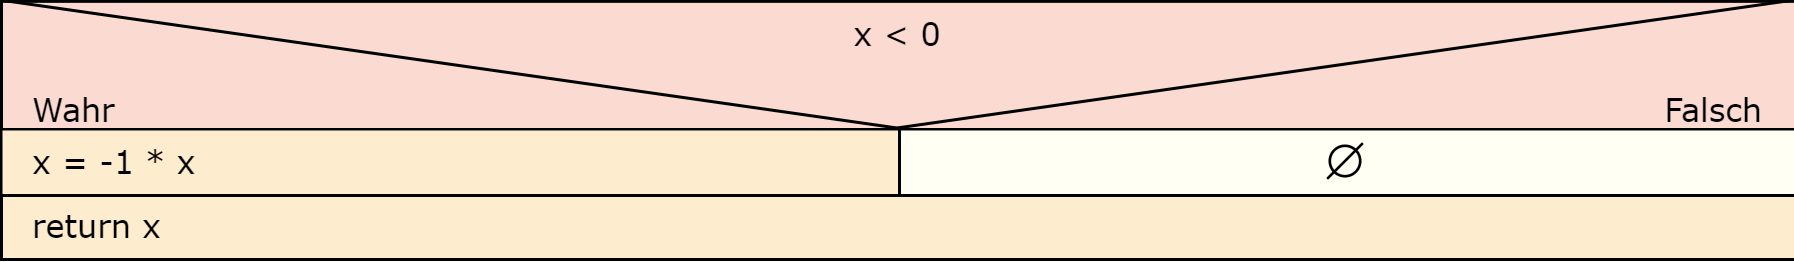
\includegraphics[width=\textwidth]{_Aufgaben/BlocksAndJava/img/strukt_betrag.png} \\\\
+ double potenzieren(double b, double p) \\
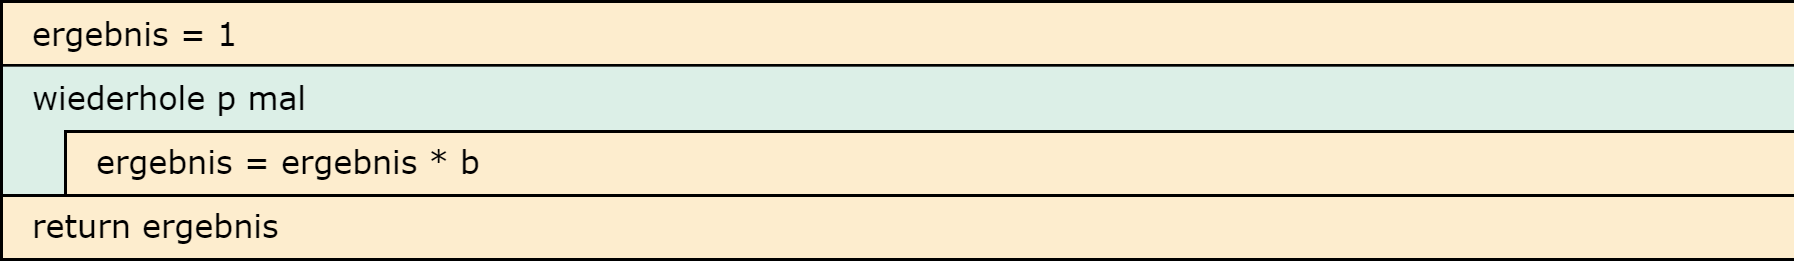
\includegraphics[width=\textwidth]{_Aufgaben/BlocksAndJava/img/strukt_protenz.png}}{25}

    
\end{minipage}


\begin{minipage}[t]{\textwidth}
\Large
\begin{lstlisting}[escapechar=\&]
public class ErweiterterTaschenrechner
{    
    public & \LoesungLuecke{double betrag(double z1) \{ }{15cm} &
    
        & \LoesungLuecke{if(z1 < 0) \{ }{15cm} &
        
            & \LoesungLuecke{z1 = -1 * z1;}{15cm} &
            
        & \LoesungLuecke{\}}{15cm} &   
        
        & \LoesungLuecke{return z1;}{15cm} &   
    }
    public & \LoesungLuecke{void piAusgeben(double x) \{ }{15cm} &
    
        & \LoesungLuecke{for(int i=0; i < x; i++) \{ }{15cm} &
        
            & \LoesungLuecke{System.out.println(Math.PI);}{15cm} &
            
        & \LoesungLuecke{\}}{15cm} &
    }
    public & \LoesungLuecke{double potenzieren(double b, double p) \{ }{15cm} &

        & \LoesungLuecke{double ergebnis = 1.0;}{15cm} &
    
        & \LoesungLuecke{for(int i=0; i < p; i++) \{ }{15cm} &
        
            & \LoesungLuecke{ergebnis = ergebnis * b;}{15cm} &
            
        & \LoesungLuecke{\}}{15cm} &
            
        & \LoesungLuecke{return ergebnis;}{15cm} &
    }
}
\end{lstlisting}

\end{minipage}